In this section, we evaluate the performance of our framework. Our
implementation is open source and can be found at \cite{sources}, which also
includes the experimental setup along with configuration files and input data.
The experiments discussed below are conducted on a \up{GNU}/Linux machine
equipped with 16 processors Intel Xeon E5520 2.27~\up{GH}z and 24~\up{GB} of
\up{RAM}.

\updated{We shall address $3 \times 2 \times 3 = 18$ uncertainty-quantification
problems. Specifically, we shall consider three platform sizes $\np$: 2, 4, and
8 processing elements; two application sizes $\nt$: 10 and 20 tasks; and three
metrics $\g$: the end-to-end delay, total energy consumption, and maximum
temperature defined in \eref{end-to-end-delay}, \eref{total-energy}, and
\eref{maximum-temperature}, respectively.} At this point, it might be helpful to
recall the example in \fref{example}.

\subsection{Configuration} \slab{configuration}
A platform with $\np$ processing elements and an application with $\nt$ tasks
are generated randomly by the \up{TGFF} tool \cite{dick1998}. The tool generates
$\np$ tables and a directed acyclic graph with $\nt$ nodes. Each table
corresponds to a processing element, and it describes certain properties of the
tasks when they are mapped to that particular processing element. Namely, each
table assigns two numbers to each task: a reference execution time, chosen
uniformly between 10 and 50~ms, and a power consumption, chosen uniformly
between 5 and 25~W. The graph captures data dependencies between the tasks. The
application is scheduled using a list scheduler \cite{adam1974}. The mapping of
the application is fixed and obtained by scheduling the tasks based on their
reference execution times and assigning them to the earliest available
processing elements (a shared ready list).

The construction of thermal \up{RC} circuits needed for temperature analysis is
delegated to the HotSpot tool \cite{skadron2004}. The floorplan of each platform
is a regular grid wherein each processing element occupies $2 \times
2~\text{mm}^2$ on the die. The output of the tool is a pair of a thermal
capacitance matrix $\mC$ and a thermal conductance $\mG$ matrix used in
\eref{thermal-system}. The leakage modeling is based on a linear fit to a data
set of \up{SPICE} simulations of a series of \up{CMOS} invertors
\cite{ukhov2012, liu2007}; see also \cite{ukhov2014}. The time step of power and
temperature profiles is constant and equal to one microsecond; see \sref{power}
and \sref{temperature}.

The uncertain parameters $\vu$ introduced in \sref{problem} are the execution
times of the tasks; see \sref{time}. All other parameters are deterministic.
Targeting the practical scenario described in \sref{parameters}, the marginal
distributions and correlation matrix of $\vu$ are assumed to be available.
Without loss of generality, the marginal of $\u_i$ is a four-parametric beta
distribution $\text{Beta}(\alpha_i, \beta_i, a_i, b_i)$ where $\alpha_i$ and
$\beta_i$ are the shape parameters, and $a_i$ and $b_i$ are the endpoints of the
support. The left $a_i$ and right $b_i$ endpoint are set to 80\% and 120\%,
respectively, of the reference execution time generated by the \up{TGFF} tool as
described earlier. The parameter $\alpha_i$ and $\beta_i$ are set to two and
five, respectively, for all tasks, which skews the corresponding distribution
toward the left endpoint. The execution times of the tasks are correlated based
on the structure of the graph produced by the \up{TGFF} tool: the closer task
$i$ and task $j$ are in the graph as measured by the number of edges between
vertex $i$ and vertex $j$, the stronger $\u_i$ and $\u_j$ are correlated. The
model-order reduction parameter $\eta$ in \eref{reduction} (\sref{parameters})
is set to 0.9, which results in $\nz = 2$ and 3 preserved variables for
applications with $\nt = 10$ and 20 tasks, respectively.

The configuration of the interpolation algorithm (the collocation nodes, basis
functions, and adaptation strategy with stopping conditions) is as described in
\sref{interpolation}. The parameters $\aerror$, $\rerror$, and $\serror$ are
around $10^3$, $10^2$, and $10^4$, respectively, depending on the problem; the
exact values can be found at \cite{sources}, which, again, contains all other
details too.

The performance of our framework with respect to each problem is assessed as
follows. \updated{First, we obtain the ``true'' probability distribution of the
metric in question $\g$ by sampling $\g$ directly and extensively.} Direct
sampling means that samples are drawn from $\g$ itself (not from a surrogate),
and that there is no any intermediate model-order reduction (see
\sref{parameters}). Second, we construct an interpolant for $\g$ and estimate
$\g$'s distribution by sampling the interpolant. In both cases, we draw $10^5$
samples; let us remind, however, that the cost of sampling the interpolant is
practically negligible. \updated{Third, we perform another round of direct
sampling of $\g$, but this time we draw as many samples as many times the metric
was evaluated during the interpolation process.} In each of the three cases, the
sampling is undertaken in accordance with a Sobol sequence, which is a
quasi-random low-discrepancy sequence featuring much better convergence
properties than those of the vanilla Monte-Carlo (\up{MC}) sampling
\cite{joe2008}.

As a result, we obtain three estimates of $\g$'s distribution: reference (the
one considered true), proposed (the one interpolation powered), and direct (the
one equal in terms of the number of $\g$'s evaluations to the proposed
solution). The last two are compared with the first one. For comparing the
proximity between two distributions, we use the well-known Kolmogorov--Smirnov
(\up{KS}) statistic \cite{rao2009}, which is the supremum over the distance
(pointwise) between two empirical distribution functions and, hence, is a rather
unforgiving error indicator.


\subsection{Discussion}
\begin{figure*}
  \vspace{-1.5em}
  \centering
  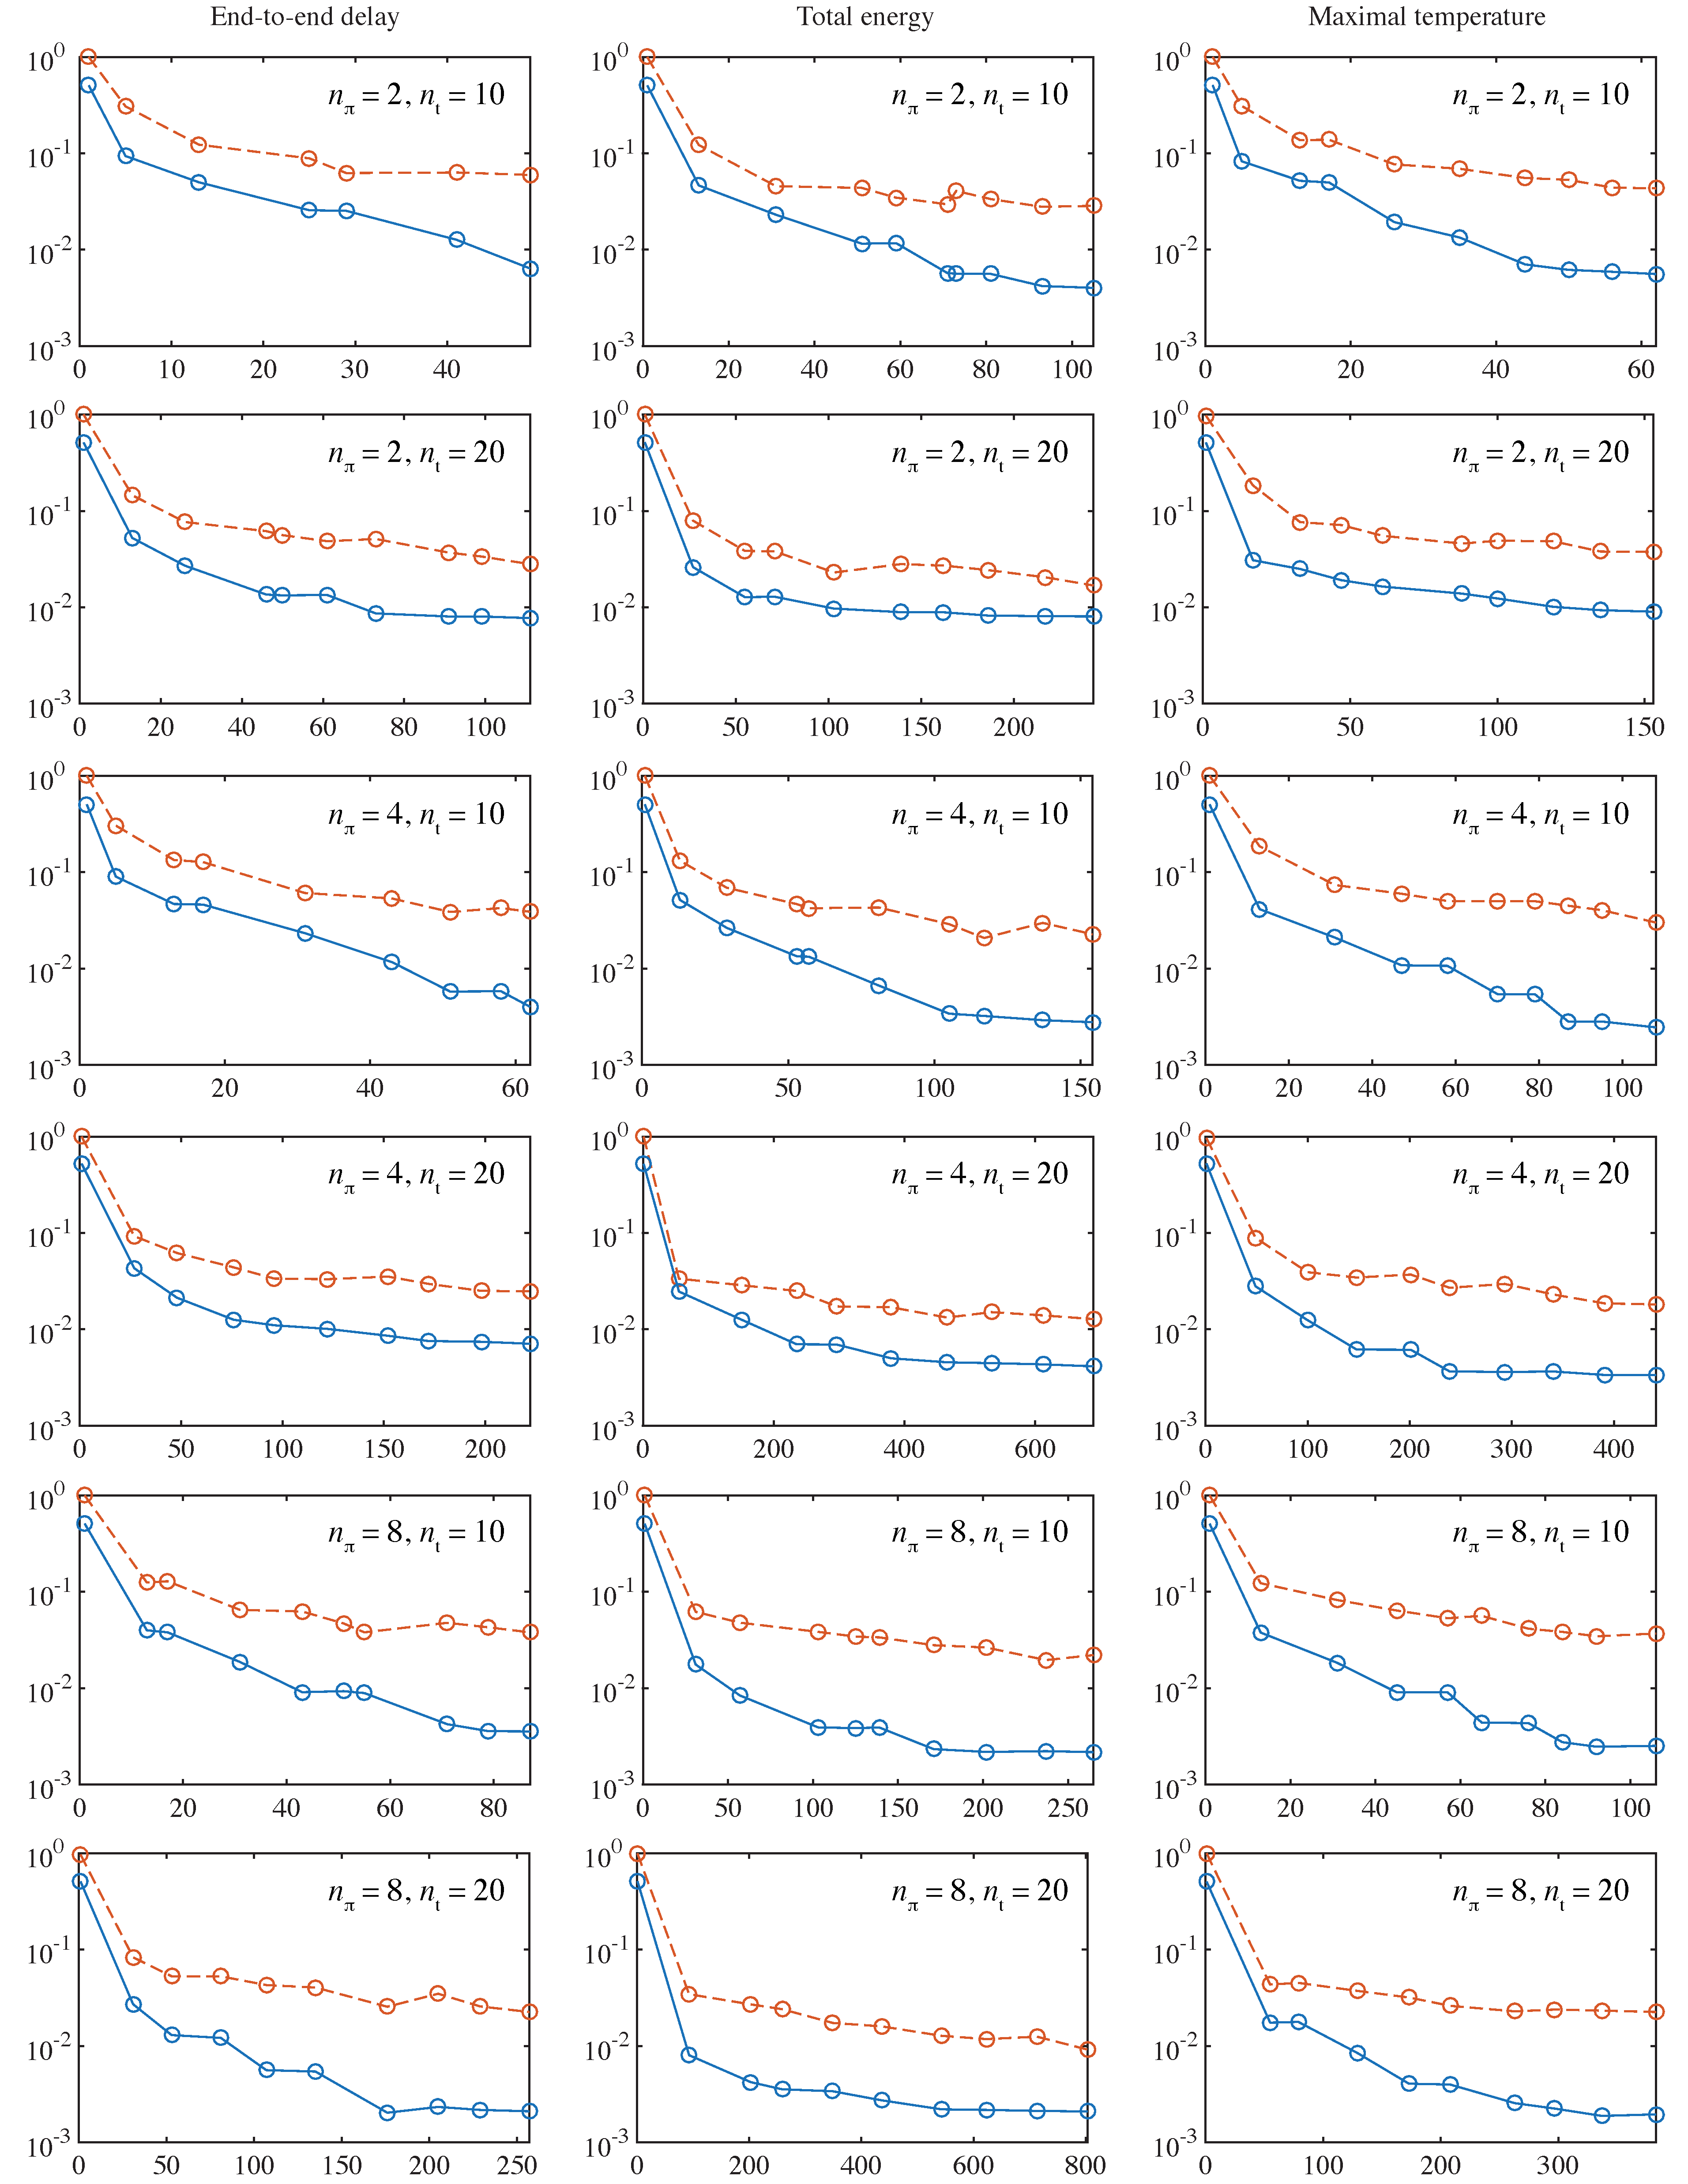
\includegraphics[width=1.0\textwidth]{include/assets/figures/results.pdf}
  \vspace{-1.5em}
  \caption{
    Experimental results. There are considered 3 platform sizes, 2 application
    sizes, and 3 quantities. The columns correspond to the three quantities: the
    end-to-end delay (left), total energy (middle), and maximum temperature
    (right). The rows alternate between the two application sizes: 10 (odd) and
    20 (even) tasks. The three pairs of rows correspond to the three platform
    sizes: 2 (top), 4 (middle), and 8 (bottom) processing elements. The
    horizontal axes show the number of points, and the vertical ones the error
    on a logarithmic scale. The solid lines correspond to our technique, and the
    dashed ones to direct sampling.
  }
  \flab{results}
\end{figure*}

The results of all 18 uncertainty-quantification problems are given in
\fref{results} as a 6-by-3 grid of plots, one plot per problem. The three
columns correspond to the three quantities of interest: the end-to-end delay
(left), total energy (middle), and maximum temperature (right). The three pairs
of rows correspond to the three platform sizes: 2 (top), 4 (middle), and 8
(bottom) processing elements. The rows alternate between the two application
sizes: 10 (odd) and 20 (even) tasks.

The horizontal axis of each plot shows the number of points, that is,
evaluations of the quantity of interest $\g$, and the vertical one shows the
\up{KS} statistic on a logarithmic scale. Each plot has two lines. The solid
line represents our technique. The circles on this line correspond to the steps
of the interpolation process given in \eref{approximation}. They show how the
\up{KS} statistic computed with respect to the reference solution changes as the
interpolation process takes steps (and increases the number of collocation
nodes) until the stopping condition is satisfied (\sref{adaptivity}). Note that
only a subset of the actual steps is displayed in order to make the figure
legible. Synchronously with the solid line (that is, for the same numbers of
$\g$'s evaluations), the dashed line shows the error of direct sampling, which,
as before, is computed with respect to the reference solution.

Studying \fref{results}, one can make a number of observations. First and
foremost, our interpolation-powered approach (solid lines) to probabilistic
analysis outperforms direct sampling (dashed lines) in all the cases. This means
that, given a fixed budget of the computation time---the probability
distributions delivered by our framework are much closer to the true ones than
those delivered by sampling $\g$ directly, despite the fact that the latter
relies on Sobol sequences, which are a sophisticated sampling strategy. Since
direct sampling methods try to cover the probability space impartially,
\fref{results} is a salient illustration of the difference between being
adaptive and nonadaptive.

It can also be seen in \fref{results} that, as the number of evaluations
increases, the solutions computed by our technique approach the exact ones. The
error of our framework decreases generally steeper than the one of direct
sampling. The decrease, however, tends to plateau toward the end of the
interpolation process (when the stopping condition is satisfied). This behavior
can be explained by the following two reasons. First, the algorithm has been
instructed to satiate certain accuracy requirements ($\aerror$, $\rerror$, and
$\serror$), and it reasonably does not do more than what has been requested.
Second, since the model-order reduction mechanism is enabled in the case of
interpolation, the quantity being interpolated is not $\g$, strictly speaking;
it is a lower-dimensional representation of $\g$, which already implies an
information loss. Therefore, there is a limit on the accuracy that can be
achieved, which depends on the amount of reduction applied. However, model-order
reduction is a good, recommended practice since it circumvents unnecessary
complexity and, thereby, makes uncertainty-quantification problems more
tractable.

Let us walk through a particular problem in \fref{results}. Consider, for
instance, the one labeled with $\bigstar$. It can be seen that our solution and
the solution of direct sampling are poor at the very beginning. The \up{KS}
statistic tells us that there are substantial mismatches between the estimates
and the reference solution. However, as the interpolant is being adaptively
refined, our error starts to rapidly decrease, and, by the end of the
interpolation process, our solution becomes approximately one order of magnitude
more accurate than the one of na\"{i}ve sampling.

The message of the above observations is that the designer of an electronic
system can benefit substantially in terms of accuracy per computation time by
switching from direct sampling to the proposed technique. If the designer's
current workhorse is the classical \up{MC} sampling, the switch might lead to
even more dramatic savings than those shown in \fref{results}. Needless to
mention that the gain is especially prominent in situations where the analysis
needs to be performed many times such as when it resides in a design-space
exploration loop.

\begin{remark}
The wall-clock time taken by the experiments is not reported in this paper
because this time is irrelevant: since the evaluation of $\g$ is time consuming
(see \sref{problem}), the number of $\g$'s evaluations is the most apposite
expense indicator. For the curious reader, however, let us give an example by
considering the problem labeled with $\clubsuit$ in \fref{results}. Obtaining a
reference solution with $10^5$ simulations in parallel on 16 processors took
around two hours. Constructing an interpolant with 383 collocation nodes took
around 30 seconds (this is also the time of direct sampling with 383 simulations
of $\g$). Evaluating the interpolant $10^5$ times took less than a second. The
relative computation cost of sampling an interpolant readily diminishes as the
complexity of $\g$ increases; contrast it with direct sampling, whose cost grows
proportional to $\g$'s evaluation time.
\end{remark}


\subsection{Real-life Example}
Last but not least, we investigate the viability of deploying the framework in a
real environment. It means that we need to couple the framework with a
battle-proven simulator used in academia and industry and let it simulate a real
application running on a real platform. The scenario we consider is the same as
the one depicted in \fref{example} except for the fact that an
industrial-standard simulator is put in place of the leftmost box, and the
metric of interest $\g$ is now the total energy. Unlike the previous examples,
there is no true solution to compare with due to the prohibitive expense of the
simulator, which is exactly why our framework is needed in such cases.

The simulator of choice is the widely used combination of Sniper
\cite{carlson2011} and McPAT \cite{li2009}. The simulated architecture is
Intel's Nehalem-based Gainestown series. The platform is configured to have
three \up{CPU}s sharing one \up{L3} cache. The simulated application is
\up{VIPS}, which is an image-processing piece of software taken from \up{PARSEC}
\cite{bienia2011}. In this scenario, \up{VIPS} applies a fixed set of operations
to a given image, and the width and height of the image to process are the
uncertain parameters $\vu$, which are assumed to be distributed uniformly within
certain ranges. All other details including the infrastructure developed for
this example can be found at \cite{sources}.

The real-life deployment has fulfilled our expectations. The interpolation
process successfully finished and delivered a surrogate after 78 invocations of
the simulator. Each invocation took 40 minutes on average. The probability
distribution of the total energy was then estimated by sampling the constructed
surrogate $10^5$ times. This many samples would take months to obtain if one
sampled the simulator directly. Using the proposed technique, the whole
procedure took several hours.

